% Loading-overlay mark: the extension's own logo — an isometric L-tromino of
% three unit cubes, the bottom-right one tetrahedralized — redrawn as a
% monochrome WIREFRAME rather than the teal-filled marketplace icon
% (icons/tikz-icon/icon.tex), so it inherits the theme foreground like every
% other icon here instead of shipping a raster asset the webview cannot reach.
%
% Coordinates are icon.tex's, translated to put the figure's centre on the
% origin and halved: the overlay ROTATES this mark, and a shape centred in its
% own viewBox turns about itself rather than orbiting.
%
% The magnifier badge is deliberately dropped — it says "preview", which is
% not what a progress indicator is about, and at this stroke weight it would
% close up into a blob. The tet split stays: it is what makes the mark read as
% a mesh rather than three boxes.
\documentclass[tikz,border=2mm]{standalone}
\begin{document}
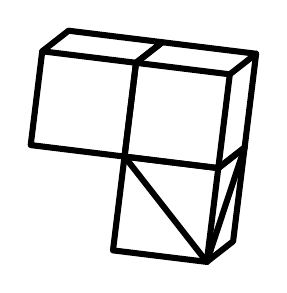
\begin{tikzpicture}[line width=2.2pt, line cap=round, line join=round, x=1mm,y=1mm, rotate=-7]
  % --- cube A (top-left) ---
  \coordinate (A-fbl) at (-13.5,-1.5);
  \coordinate (A-fbr) at (-1.5,-1.5);
  \coordinate (A-ftr) at (-1.5,10.5);
  \coordinate (A-ftl) at (-13.5,10.5);
  \coordinate (A-btr) at (1.5,13.5);
  \coordinate (A-btl) at (-10.5,13.5);
  % --- cube B (top-right) ---
  \coordinate (B-fbl) at (-1.5,-1.5);
  \coordinate (B-fbr) at (10.5,-1.5);
  \coordinate (B-ftr) at (10.5,10.5);
  \coordinate (B-ftl) at (-1.5,10.5);
  \coordinate (B-bbr) at (13.5,1.5);
  \coordinate (B-btr) at (13.5,13.5);
  \coordinate (B-btl) at (1.5,13.5);
  % --- cube C (bottom-right, tetrahedralized) ---
  \coordinate (C-fbl) at (-1.5,-13.5);
  \coordinate (C-fbr) at (10.5,-13.5);
  \coordinate (C-ftr) at (10.5,-1.5);
  \coordinate (C-ftl) at (-1.5,-1.5);
  \coordinate (C-bbr) at (13.5,-10.5);
  \coordinate (C-btr) at (13.5,1.5);

  % === edges — only genuinely exterior faces, as in the icon ===
  \draw (A-fbl) -- (A-fbr) -- (A-ftr) -- (A-ftl) -- cycle;
  \draw (A-ftl) -- (A-btl) -- (A-btr) -- (A-ftr);

  \draw (B-fbl) -- (B-fbr) -- (B-ftr) -- (B-ftl) -- cycle;
  \draw (B-ftl) -- (B-btl) -- (B-btr) -- (B-ftr);
  \draw (B-fbr) -- (B-bbr) -- (B-btr);

  \draw (C-fbl) -- (C-fbr) -- (C-ftr) -- (C-ftl) -- cycle;
  \draw (C-fbr) -- (C-bbr) -- (C-btr) -- (C-ftr);

  % === cube C tet split: fan from C-fbr, the vertex its two visible faces share ===
  \draw (C-fbr) -- (C-ftl);
  \draw (C-fbr) -- (C-btr);
\end{tikzpicture}
\end{document}
